\subsection{Dataset}
	We implemented our own crawler in Java, and collected video information from October 1st to November 5th, 2014, with several stops and updates.  We then crawled the corresponding uploader data. The crawling strategy is akin to bread-first search. First we initialize the crawler with several random "seed" videos, which mostly are in the \textit{Movie} and \textit{Music} category, and recursively explore all other videos that YouTube suggests are related to those videos. For each video, we extract all of its metadata such as title, uploader, description, upload date, number of views/likes/dislikes, video length, and a number of other attributes, as well as a list of around 30 videos YouTube recommends as being similar.  The data crawling was a very significant part of our project.

	\subsubsection{Data Statistics}
		Although the crawler was suspended twice due to technical issues and upgrades, we have gathered a sizable amount of data, with tremendous  variation in the observed values:

		\begin{itemize}
			\item Number of videos crawled: 1,432,213
			\item Number of uploaders: 628,072
			\item Most viewed video: 2,104,518,656 views.
			\item Most "liked" video: 8,639,650 likes.
			\item Most "disliked" video: 4,184,769 dislikes.
			\item Size of "bag of words" dictionary produced for the titles and descriptions: 2,447,603 entries.
		\end{itemize}

		We plot in Figure \ref{fig:logNoOfViews} the distribution of number of views in our current data. Interestingly, the distribution is in the shape of Gaussians, instead of following the Power Law distribution as frequently observed in social networks. We guess that this observation is due to the way we sampled the data, by following the recommended links: This would imply that popularity of a video is one of the most important factors in the YouTube recommender systems. Whether we can uncover the underlying reasons of links suggested by YouTube, namely, based on similarity or popularity or both, is an interesting question and may be addressed in our future work.
		
		As the statistics show, we have a large magnitude in ranges of number of view, likes and dislikes. This motivates us to do some preprocessing on data, such as feature normalization or data standardization, to ensure the numerical stability and good speed of convergence on the learning algorithm for logistic regression. We discuss more on this step in the Section \ref{sec:orderofmagnitude}.
		
		\begin{figure}[!h]
			\begin{center}
				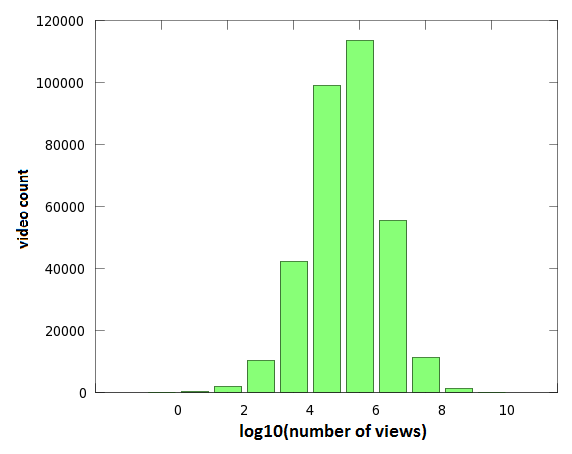
\includegraphics[width=.75\textwidth,clip]{DistributionOfViews.png}
			\end{center}
			\caption{Histogram on the distribution of number of views (in log-scale).}
			\label{fig:logNoOfViews}
		\end{figure}
				
	\subsubsection{Feature extraction}
		The first step is to build a dictionary mapping the uploader to the number of videos they have uploaded and the total number of views there videos have. We also take care to prevent "cheating":  In order to ensure that our predictor has only such information as would be available before the video's publishing is ever used, we temporarily reduce these number of video-views and the total number of video uploads for the uploader according to the publish date of the video under current consideration.

		We considered many features, which ultimately include:
		\begin{itemize}
			\item
			Features extracted via a bag-of-words model on the title, using TF-IDF.
			\item
			The number of videos uploaded by the uploader prior to the current video's upload date.  Because of our desire for caution against "cheating", we count only those videos that we have crawled.
			\item
			The total number of views for the uploader due to videos released prior to the current video's upload date.  Again, we count only those videos that we have crawled.  This date-conscious counting is particularly important because there are many cases where there is only one video crawled for a given uploader, meaning that this feature would become a nearly perfect predictor.
			\item
			The number of subscribers for the uploader.  We lack sufficient data to know how subscribers changed over time, so we simply had to keep this constant.
			\item
			The runtime of the video, in seconds.
			\item
			The age of the video at the time of crawling, in days.
			\item
			The number of likes/dislikes.  Since these are expected to scale with the number of views, we forbade ourselves from using the number directly, but we did allow certain combinations, such as the log of the like-vs-dislike ratio.
			\item
			Various combinations of the above features (for example, the log of some other feature, or the ratio between two features).
		\end{itemize}
	
\subsection{Evaluation Metrics}
	Two evaluation measures widely used to evaluate ranking approaches are the 0-1 loss function, Area under Curve (AUC). The \textbf{0-1 loss function} is the ratio of correctly ordered video pairs over total number of pairs in testing set.
	\begin{equation}
		0/1_{loss} = \sum_{(u, v)_{test}} \frac{1}{|(u,v)_{test}|} \textbf{1}[\hat{Y}_{uv} - Y_{uv} == 0]
	\end{equation}
	Since our label values are all in the set \{0, 1\}, we can also use  \textbf{AUC Loss} as another ranking-based performance metric.
	\begin{equation}
		AUC_{loss} = 1 - AUC,
	\end{equation}
	where AUC is the area under the ROC curve.
